\begingroup
\newcolumntype{L}[1]{>{\hsize=#1\hsize\raggedright\arraybackslash}X}

\section{Hình ảnh minh chứng bắt buộc}
\label{sec:evidence}
Phần này lưu trữ ảnh chụp trạng thái trước và sau khi cấu hình Router/AP, thông
tin kết nối của Laptop, Desktop, Smartphone và minh chứng kiểm tra Ad-hoc tối
thiểu hai node ping được nhau. Ảnh minh chứng của mô hình Ad-hoc đã được nhóm
thu thập đầy đủ và trình bày ở Mục~\ref{subsec:evidence-adhoc}; ảnh minh chứng
cấu hình Router/AP và kết nối thiết bị vật lý vẫn đang chờ nhóm bổ sung. Trước
khi đưa ảnh vào báo cáo phải che mật khẩu, địa chỉ quản trị nhạy cảm và dữ liệu
cá nhân.

\subsection{Minh chứng cấu hình Router/AP và kết nối thiết bị}
\label{subsec:evidence-infra}

\begin{figure}[htbp]
  \centering
  \fbox{\parbox[c][4cm][c]{0.85\linewidth}{\centering
    Để trống -- chèn ảnh minh chứng cấu hình Router/AP}}
  \caption{Minh chứng cấu hình Router/AP (nhóm bổ sung ảnh thực tế)}
  \label{fig:evidence-router}
\end{figure}

\begin{figure}[htbp]
  \centering
  \fbox{\parbox[c][4cm][c]{0.85\linewidth}{\centering
    Để trống -- chèn ảnh kết nối Laptop, Desktop và Smartphone}}
  \caption{Minh chứng kết nối thiết bị đầu cuối (nhóm bổ sung ảnh thực tế)}
  \label{fig:evidence-clients}
\end{figure}

\subsection{Minh chứng mô hình Ad-hoc (IBSS) hai nút}
\label{subsec:evidence-adhoc}

Trước hết, khả năng hỗ trợ của hệ điều hành được kiểm tra trên máy chủ vật lý
chạy Windows~11. Lệnh \texttt{netsh wlan show drivers} trả về dòng
\emph{Hosted network supported: No} (Hình~\ref{fig:win-hosted}), xác nhận rằng
nền tảng Windows không còn hỗ trợ chế độ ngang hàng, phù hợp với nhận định trong
Mục~\ref{sec:arch}. Vì vậy mạng Ad-hoc được triển khai trên Linux theo quy trình
tại Mục~\ref{sec:adhoc-config}.

\begin{figure}[htbp]
  \centering
  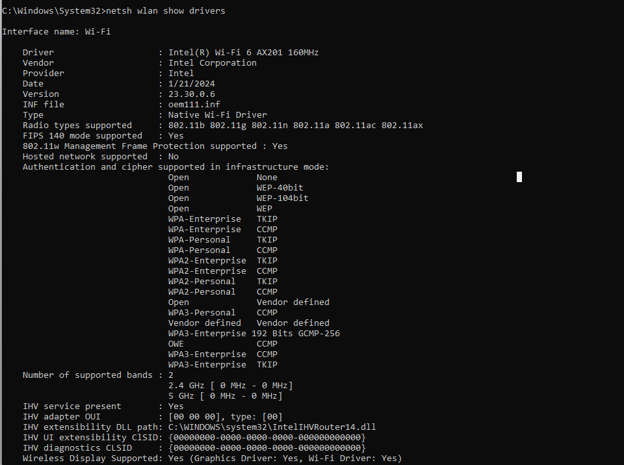
\includegraphics[width=\linewidth]{figures/Picture1.png}
  \caption{Kết quả \texttt{netsh wlan show drivers} trên Windows~11 với dòng
  ``Hosted network supported: No'', cho thấy hệ điều hành không hỗ trợ chế độ
  Ad-hoc.}
  \label{fig:win-hosted}
\end{figure}

Hai card mạng không dây ảo được tạo bằng module \texttt{mac80211\_hwsim} với
tham số \texttt{radios=2}. Kết quả \texttt{iw dev}
(Hình~\ref{fig:hwsim-radios}) xuất hiện hai radio độc lập \texttt{phy\#0} và
\texttt{phy\#1} cùng hai giao diện \texttt{wlan0}, \texttt{wlan1}; giao diện
\texttt{P2P-device} đi kèm \texttt{phy\#1} do trình điều khiển tự tạo để phục vụ
Wi-Fi Direct và không ảnh hưởng đến kết nối Ad-hoc.

\begin{figure}[htbp]
  \centering
  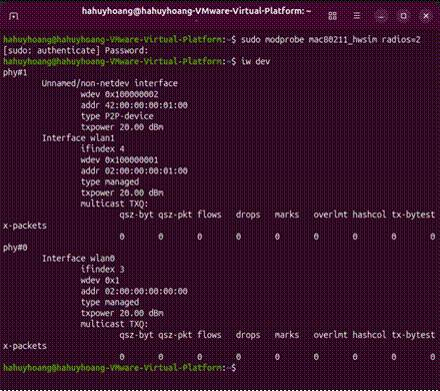
\includegraphics[width=\linewidth]{figures/Picture2.png}
  \caption{Kết quả \texttt{iw dev} sau khi nạp module
  \texttt{mac80211\_hwsim radios=2}: hai radio ảo \texttt{phy\#0} (wlan0) và
  \texttt{phy\#1} (wlan1) được khởi tạo.}
  \label{fig:hwsim-radios}
\end{figure}

Để hai giao diện không dùng chung bảng định tuyến và chuyển gói qua loopback,
mỗi radio được tách vào một network namespace riêng (Hình~\ref{fig:netns}), nhờ
đó mỗi radio hoạt động như một máy tính độc lập.

\begin{figure}[htbp]
  \centering
  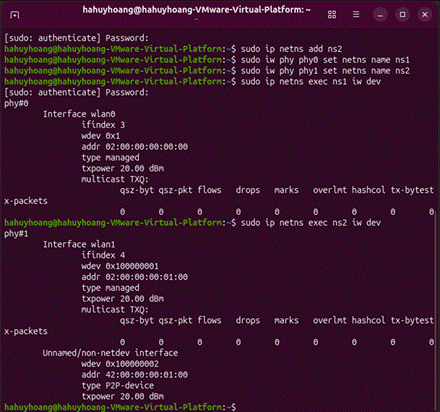
\includegraphics[width=\linewidth]{figures/Picture3.png}
  \caption{Mỗi radio được gán vào một network namespace riêng: \texttt{ns1} chỉ
  thấy \texttt{phy\#0}, \texttt{ns2} chỉ thấy \texttt{phy\#1}.}
  \label{fig:netns}
\end{figure}

Hai nút được chuyển sang chế độ \ac{ibss}, cùng tham gia mạng
\texttt{demoAdhoc} trên tần số 2437~MHz (kênh~6) và được gán địa chỉ
\texttt{10.0.0.1/24}, \texttt{10.0.0.2/24} (Hình~\ref{fig:adhoc-config}).

\begin{figure}[htbp]
  \centering
  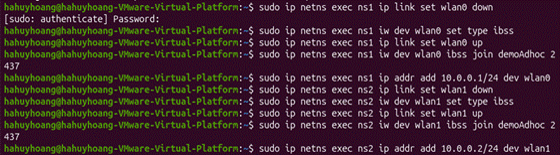
\includegraphics[width=\linewidth]{figures/Picture4.png}
  \caption{Chuỗi lệnh cấu hình chế độ IBSS cho Node~1 (\texttt{ns1},
  \texttt{wlan0}) và Node~2 (\texttt{ns2}, \texttt{wlan1}).}
  \label{fig:adhoc-config}
\end{figure}

Kết quả kiểm tra ở Hình~\ref{fig:adhoc-check} cho thấy \texttt{wlan0} đang ở
\texttt{type IBSS}, \ac{ssid} \texttt{demoAdhoc}, kênh~6 (2437~MHz), độ rộng
20~MHz; lệnh \texttt{station dump} ghi nhận nút còn lại với MAC
\texttt{02:00:00:00:01:00} đã ở trạng thái \emph{authorized} và
\emph{associated}, tức hai nút đã nhận ra nhau ở tầng 802.11.

\begin{figure}[htbp]
  \centering
  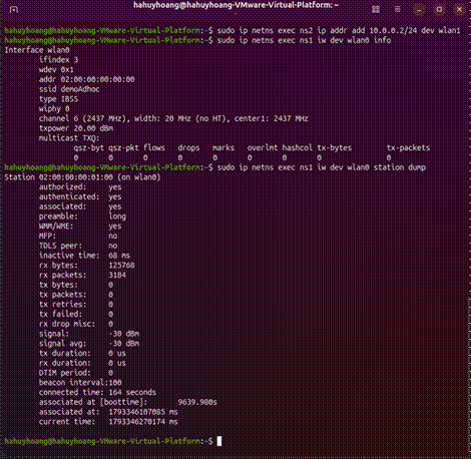
\includegraphics[width=\linewidth]{figures/Picture5.png}
  \caption{Kết quả \texttt{iw dev wlan0 info} (type IBSS, ssid demoAdhoc, kênh~6)
  và \texttt{station dump} (nút lân cận \texttt{02:00:00:00:01:00} đã
  authenticated và associated).}
  \label{fig:adhoc-check}
\end{figure}

Cuối cùng, lệnh ping bốn gói từ Node~1 sang Node~2
(Hình~\ref{fig:adhoc-ping}) nhận đủ 4/4 phản hồi, tỉ lệ mất gói 0\,\%, chứng
minh mạng Ad-hoc đã hoạt động ở cả tầng liên kết dữ liệu và tầng mạng.

\begin{figure}[htbp]
  \centering
  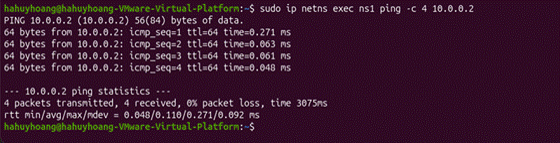
\includegraphics[width=\linewidth]{figures/Picture6.png}
  \caption{Kết quả \texttt{ping -c 4 10.0.0.2} từ Node~1 sang Node~2: 4 gói gửi,
  4 gói nhận, mất gói 0\,\%.}
  \label{fig:adhoc-ping}
\end{figure}

\clearpage
\section{Kết quả thử nghiệm và thảo luận}
\label{sec:experiment}

\subsection{Mục tiêu và phạm vi thử nghiệm}
Mục tiêu của phần thử nghiệm là kiểm chứng bằng thực nghiệm hai nội dung lý
thuyết đã trình bày: (i) mô hình Ad-hoc (IBSS) cho phép hai thiết bị đầu
cuối liên lạc trực tiếp với nhau mà không cần \ac{ap}; (ii) mô hình hạ tầng là
điều kiện cần để các thiết bị đầu cuối truy cập mạng ngoài và sử dụng bảo mật
hiện đại. Trong phạm vi báo cáo lần này, nhóm hoàn thành phần (i) trên nền Linux
ảo hóa; phần (ii) với Router/AP và các thiết bị Laptop, Desktop, Smartphone vật
lý đang được tiếp tục thực hiện và sẽ được cập nhật vào các mục còn để trống
dưới đây.

\subsection{Thiết bị và mô hình thử nghiệm}
Môi trường thử nghiệm của mô hình Ad-hoc được tóm tắt trong
Bảng~\ref{tab:adhoc-env}.

\begin{table}[htbp]
  \centering\footnotesize
  \caption{Môi trường và tham số thử nghiệm mạng Ad-hoc (IBSS).}
  \label{tab:adhoc-env}
  \begin{tabularx}{\linewidth}{@{} L{0.7} L{1.3} @{}}
    \toprule
    \textbf{Hạng mục} & \textbf{Giá trị đã sử dụng} \\
    \midrule
    Máy chủ (host) & Windows~11, kiểm tra hỗ trợ bằng \texttt{netsh wlan show drivers} \\
    Máy ảo & Ubuntu 22.04 LTS Desktop trên VMware Workstation/Player \\
    Card mạng vô tuyến & 02 card ảo do module \texttt{mac80211\_hwsim} sinh ra
      (\texttt{phy\#0}, \texttt{phy\#1}) \\
    Cách ly mạng & 02 network namespace (\texttt{ns1}, \texttt{ns2}), mỗi
      namespace giữ một radio \\
    \ac{ssid} và tần số & \texttt{demoAdhoc}, 2437~MHz (kênh~6), độ rộng 20~MHz \\
    Địa chỉ IP & \texttt{10.0.0.1/24} (Node~1) và \texttt{10.0.0.2/24} (Node~2) \\
    Bảo mật & Mạng mở (không \ac{wep}, không WPA2/WPA3) \\
    \bottomrule
  \end{tabularx}
\end{table}

\subsection{Quy trình và kết quả kiểm tra}
Quy trình cấu hình gồm năm bước được trình bày tại Mục~\ref{sec:adhoc-config};
kết quả kiểm tra tổng hợp ở Bảng~\ref{tab:adhoc-results}.

\begin{table}[htbp]
  \centering\footnotesize
  \caption{Kết quả kiểm tra mạng Ad-hoc hai nút.}
  \label{tab:adhoc-results}
  \begin{tabularx}{\linewidth}{@{} L{0.8} L{0.9} L{1.3} @{}}
    \toprule
    \textbf{Nội dung kiểm tra} & \textbf{Lệnh} & \textbf{Kết quả quan sát} \\
    \midrule
    Giao diện ở chế độ Ad-hoc & \texttt{iw dev wlan0 info} &
      \texttt{type IBSS}, \ac{ssid} \texttt{demoAdhoc}, kênh~6 (2437~MHz), độ
      rộng 20~MHz \\
    Phát hiện nút lân cận & \texttt{station dump} &
      MAC \texttt{02:00:00:00:01:00}, \emph{authorized} và \emph{associated} bằng
      \emph{yes}, cường độ tín hiệu $-30$~dBm, chu kỳ beacon 100~ms \\
    Liên lạc ở tầng mạng & \texttt{ping -c 4 10.0.0.2} &
      4 gói gửi, 4 gói nhận, mất gói 0\,\%; RTT nhỏ nhất/trung bình/lớn
      nhất/độ lệch là 0,048 / 0,110 / 0,271 / 0,092~ms \\
    \bottomrule
  \end{tabularx}
\end{table}

Hai nút đã nhận diện được nhau ở tầng 802.11 và trao đổi thành công gói ICMP,
đáp ứng yêu cầu tối thiểu ``Ad-hoc có ít nhất hai node ping được nhau''. Các
bước chuyển chế độ, tham gia \ac{ibss} và gán địa chỉ IP đều thực hiện được mà
không cần bất kỳ \ac{ap} nào, đúng với mô tả kiến trúc ở
Mục~\ref{sec:arch}.

\subsection{Thảo luận, hạn chế và hướng khắc phục}
\begin{itemize}[leftmargin=*]
  \item \textbf{Độ trễ rất thấp nhưng không đại diện cho Wi-Fi thật:}
    \texttt{mac80211\_hwsim} truyền khung bằng phần mềm ngay trong nhân hệ điều
    hành, không có độ trễ vô tuyến thực tế, nên giá trị RTT cỡ 0,05--0,27~ms chỉ
    chứng minh đường truyền logic hoạt động, không dùng để so sánh với Wi-Fi vật
    lý.
  \item \textbf{Không mô phỏng được khoảng cách, suy hao và di chuyển:} môi
    trường ảo không biểu diễn được suy hao tín hiệu theo khoảng cách hay sự di
    chuyển của nút, vì vậy các đặc tính vùng phủ, tốc độ dữ liệu và chuyển vùng
    chưa được đánh giá.
  \item \textbf{Không có DHCP:} do \ac{ibss} không có máy chủ tập trung, địa chỉ
    IP phải gán tĩnh; trong mạng nhiều nút việc này khó duy trì và dễ xảy ra
    trùng địa chỉ.
  \item \textbf{Hạn chế bảo mật:} thử nghiệm chỉ chạy ở mạng mở vì \ac{ibss}
    không hỗ trợ WPA2/WPA3; điều này khẳng định thêm nhận định ở
    Mục~\ref{sec:arch} rằng mô hình Ad-hoc không phù hợp cho dữ liệu nhạy cảm.
  \item \textbf{Chưa thử đa chặng:} mới kiểm chứng một chặng giữa hai nút; mô
    hình MANET nhiều chặng với giao thức định tuyến (AODV, DSR, OLSR) chưa được
    thử.
  \item \textbf{Hướng khắc phục:} triển khai lại trên hai máy Linux thật có card
    không dây hỗ trợ \ac{ibss} để đo thông lượng bằng \texttt{iperf3} và đo suy
    hao theo khoảng cách; bổ sung thử nghiệm Wi-Fi Direct để so sánh với Ad-hoc
    truyền thống; hoàn tất phần cấu hình Router/AP và kết nối thiết bị vật lý để
    đối chiếu hai mô hình trên cùng một môi trường.
\end{itemize}

\endgroup
